\section{Mathematical Model of Infiltration}

\begin{frame}
	\frametitle{\secname}

	\begin{block}{Richards equation 1D}
		Derived the conservation of mass,
		the one-dimensional continuity equation of infiltration is given as
		\begin{equation}\label{eq:reynoldstheorem}
			\frac{\partial\theta}{\partial t}+
			\nabla\cdot\vec{q}=0.
		\end{equation}
		By Darcy's law, $q_{z}$ represents
		\begin{equation}\label{eq:darcy}
			q_{z}=
			-K\frac{\partial H}{\partial z}=
			-K\frac{\partial(h-z)}{\partial z}=
			K\left(1-\frac{\partial h}{\partial z}\right).
		\end{equation}
		Joining the equations~\eqref{eq:reynoldstheorem} and~\eqref{eq:darcy}
		we obtain the mixed Richards formulation
		\begin{equation*}
			\frac{\partial\theta}{\partial t}+
			\frac{\partial}{\partial z}
			\left[K\left(1-\frac{\partial h}{\partial z}\right)\right]=0.
		\end{equation*}
		where\vspace*{-0.4cm}
		\begin{multicols}{2}
			\begin{itemize}
				\item $\theta$ is the soil water content $\left(m^3/m^{-3}\right)$.
				      % \item $t$ is the time
				\item $z$ is the soil depth
				\item $\vec{q}$ is the water infiltration rate $\left(m/s\right)$.
				\item $K$ is hydraulic conductivity.
				\item $H$ is the total water potential in axis $z$.
				\item $h$ is the preassure head.
			\end{itemize}
		\end{multicols}
	\end{block}
	% $$
	% 	\left\{\begin{array}{l}
	% 		C(\theta)=\frac{\partial \theta}{\partial h} \\
	% 		D(\theta)=\frac{K}{C(\theta)}=\frac{K}{\frac{\partial \theta}{\partial h}}=K \frac{\partial h}{\partial \theta}
	% 	\end{array}\right.
	% $$

	% $$
	% 	\begin{gathered}
	% 		\frac{\partial \theta}{\partial t}=\frac{\partial}{\partial z}\left(D(\theta) \frac{\partial \theta}{\partial z}\right)-\frac{\partial K}{\partial z} \\
	% 		q(t)=-D \frac{\partial \theta}{\partial z}+K(\theta)
	% 	\end{gathered}
	% $$
\end{frame}

\begin{frame}
	\frametitle{\secname}
	\begin{minipage}{0.5\textwidth}
		\begin{figure}[ht!]
			\centering
			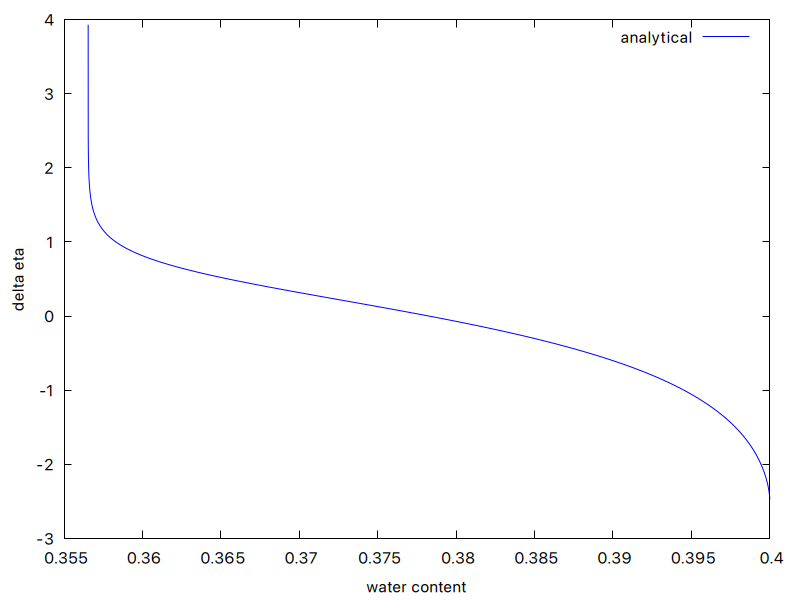
\includegraphics[width=7.2cm]{infiltration_theta_vs_deltaeta}
		\end{figure}
	\end{minipage}
	\begin{minipage}{0.3\textwidth}
		\begin{figure}[ht!]
			\centering
			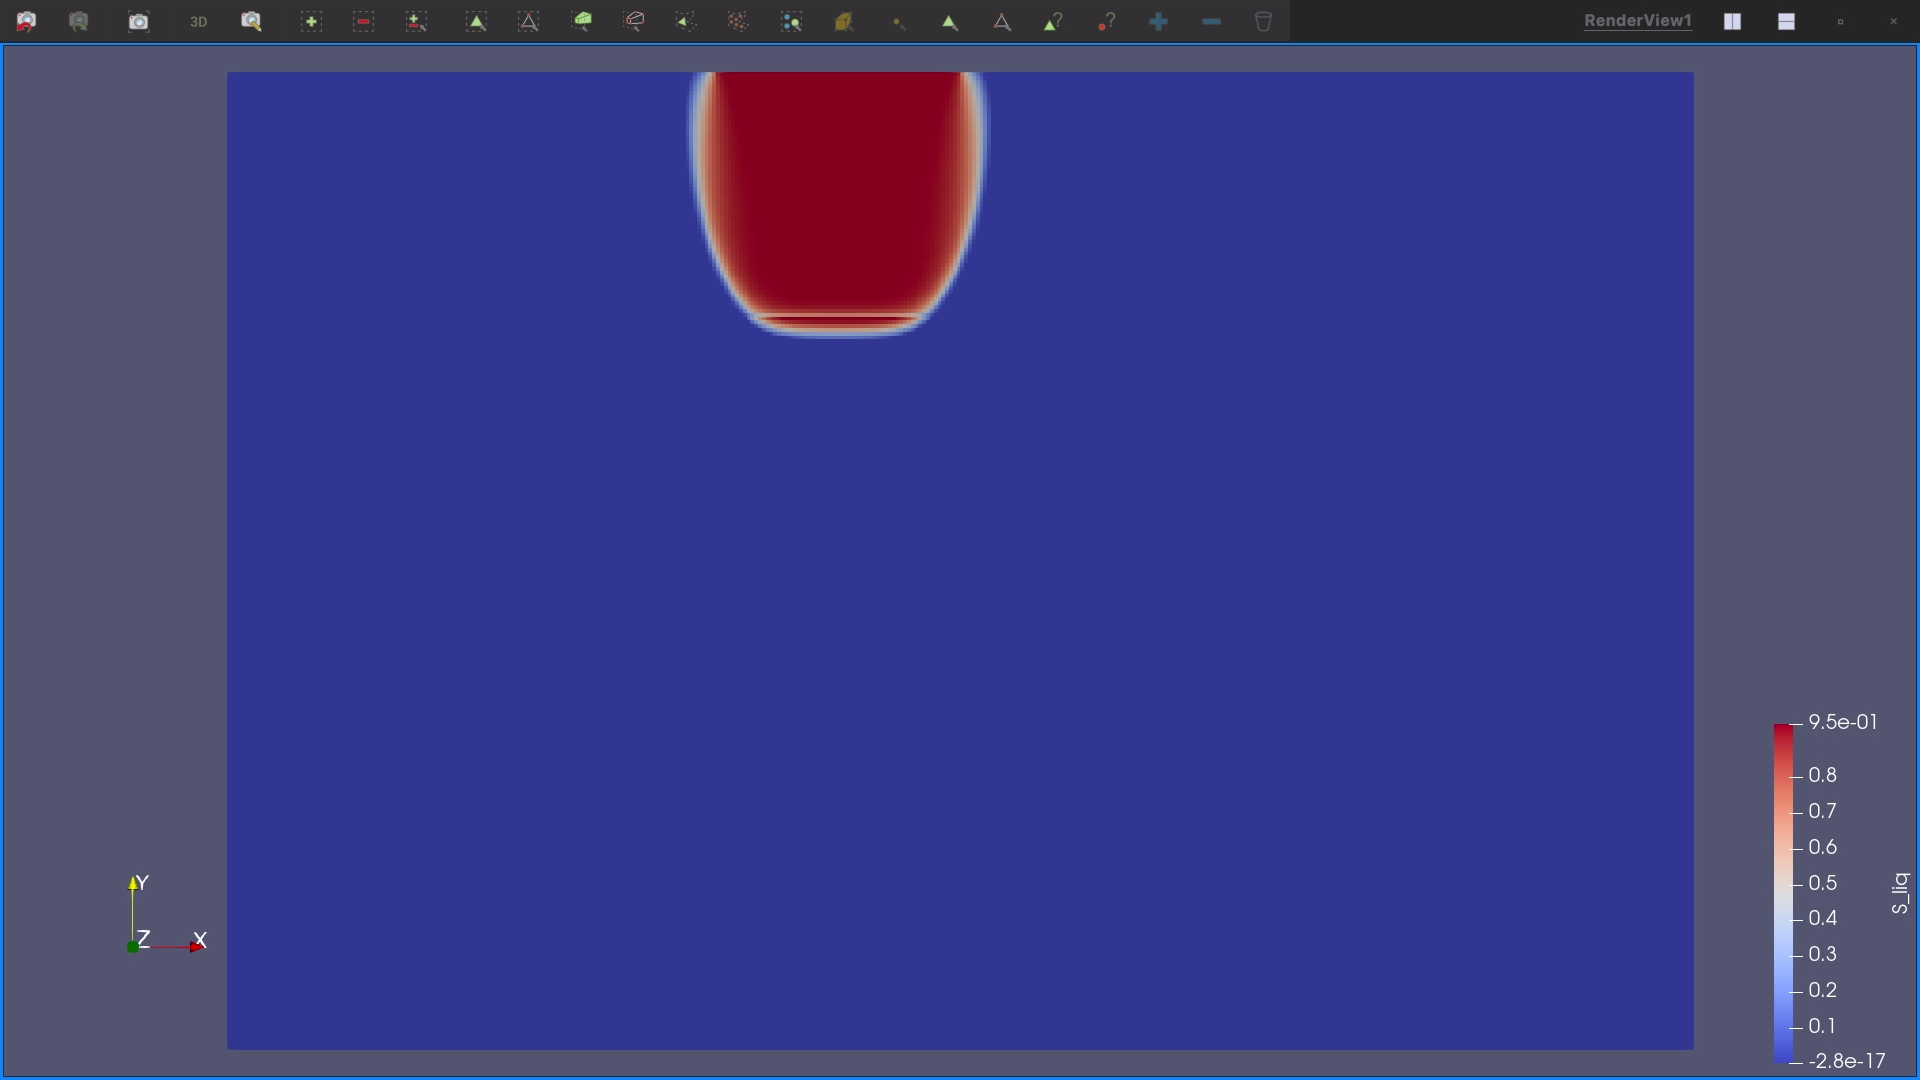
\includegraphics[width=7.2cm]{richard_lens}
		\end{figure}
	\end{minipage}
\end{frame}

% La variación de la humedad respecto al tiempo es contraria
% a la razón de cambio de infiltración con respeto a la profundidad.
% en la superficie hay más humedad y hay menos infiltración
% y a medida que avanza en el perfil del eje Z, más profundidad
% La tasa o velocidad de infiltración es la velocidad con la que el
% agua penetra en el suelo a través de su superficie.
% Normalmente la expresamos en mm/h y su valor máximo coincide con la
% conductividad hidráulica del suelo saturado